\documentclass[12pt,a4paper]{report}
\usepackage[a4paper,margin=25mm]{geometry}
\usepackage[T1]{fontenc}
\usepackage{newtxtext,newtxmath}
\usepackage{setspace}
\usepackage{graphicx}
\usepackage{float}
\usepackage{booktabs,tabularx,longtable,array}
\usepackage{enumitem}
\usepackage{tikz}
\usetikzlibrary{arrows.meta,positioning,shapes.geometric,fit}
\usepackage{xcolor}
\usepackage{hyperref}
\usepackage{caption}
\usepackage{fancyhdr}
\usepackage{titlesec}
\hypersetup{colorlinks=true,linkcolor=black,citecolor=black,urlcolor=blue,pdftitle={Chronicle: Digital Forensic Investigation and User Attribution in a Simulated Cybersecurity Incident},pdfauthor={Neil, Shreya, Aarohi}}
\setstretch{1.35}
\setlength{\parindent}{1.25cm}
\setlength{\parskip}{3pt}
\setlength{\headheight}{15pt}
\setcounter{secnumdepth}{3}
\setcounter{tocdepth}{2}
\pagestyle{fancy}
\fancyhf{}
\fancyhead[L]{Chronicle | Cyber Forensics \& Laws IA}
\fancyhead[R]{Sem V, 2026--27}
\fancyfoot[C]{\thepage}
\renewcommand{\headrulewidth}{0.4pt}
\titleformat{\chapter}[display]{\bfseries\Large}{\chaptername\ \thechapter}{8pt}{\LARGE}
\newcommand{\todo}[1]{\textcolor{red}{\textbf{[TO COMPLETE: #1]}}}
\newcommand{\caseid}[1]{\texttt{#1}}
\newcolumntype{Y}{>{\raggedright\arraybackslash}X}
\begin{document}
\begin{titlepage}
\begin{center}
\vspace*{12mm}
{\Large\bfseries SOMAIYA VIDYAVIHAR UNIVERSITY}\\[3mm]
{\large\bfseries Department of Computer Engineering}\\[18mm]
{\Large Cyber Forensics \& Laws}\\[2mm]
{\large Internal Assessment Project Report}\\[17mm]
\rule{\textwidth}{1.2pt}\\[5mm]
{\Huge\bfseries Chronicle}\\[3mm]
{\LARGE Digital Forensic Investigation and User Attribution\\in a Simulated Cybersecurity Incident}\\[5mm]
\rule{\textwidth}{1.2pt}\\[16mm]
\begin{tabular}{rl}
Course code: & 216H02C501\\
Programme / semester: & CSE (Honors), T.Y. B.Tech., Semester V\\
Academic year: & July--November 2026\\
Submitted to: & Mr Zaheed Shaikh\\
\end{tabular}\\[14mm]
\textbf{Submitted by}\\[4mm]
\begin{tabular}{lll}
Neil & \todo{Roll number} & Group member\\
Shreya & \todo{Roll number} & Group member\\
Aarohi & \todo{Roll number} & Group member\\
\end{tabular}\\[14mm]
{\large K J Somaiya School of Engineering}\\
{\large Somaiya Vidyavihar University}\\[8mm]
\todo{Verify institution, department, instructor spelling and fill roll numbers against the current course records}
\end{center}
\end{titlepage}

\pagenumbering{roman}
\chapter*{Declaration}
We submit this report for the Cyber Forensics \& Laws Internal Assessment. The report distinguishes public practice material, synthetic demonstration records, supplied screenshots, and observations produced by the current application. It does not claim that the public packet capture belongs to a real incident or to case C-001. Individual implementation responsibilities are not assigned here unless established by project records. The team members should review the final report and confirm its contents before submission.

\vspace{15mm}
\noindent Neil \hfill Shreya \hfill Aarohi\\[8mm]
\noindent Signature: \todo{Signatures if required by faculty}\\[5mm]
\noindent Date: \todo{Submission date}
\tableofcontents
\listoffigures
\clearpage
\pagenumbering{arabic}

\chapter*{Abstract}
\addcontentsline{toc}{chapter}{Abstract}
Chronicle is a local, explainable digital-forensics demonstration workbench. This report evaluates its existing pipeline using three explicitly separated tracks: a six-record synthetic regression demonstration, a 240-record synthetic Operation Glasshouse scenario, and a 43-frame public HTTP/DNS practice capture. The network case is the primary demonstration because it builds on Shreya's contributed capture, Wireshark notes and screenshots, and evidence-integrity materials. The capture is examined with tcpdump to create a structured observation export; Chronicle validates the export against the current capture fingerprint, builds a timeline, applies a DNS query/response correlation rule, and generates a report with source frame references. The resulting informational lead links frames 13 and 17 by transaction ID and reversed endpoints. It does not establish malicious activity, causation, identity, or a connection to C-001. Chronicle does not parse PCAP bytes natively, and the supplied Autopsy screenshot is not a structured filesystem examination. Synthetic cases demonstrate event processing and rule behavior, not real-world ground truth. This report documents the method, observed results, traceability, limitations, setup, and a reproducible demonstration plan.

\noindent\textbf{Keywords:} digital forensics, network evidence, provenance, timeline, correlation, SHA-256, explainability

\chapter{Introduction}
Digital investigations require more than a dashboard of alerts. An examiner needs to know what source material was examined, how records were derived, which timestamps and identifiers support a statement, what rule connected them, and what the evidence cannot establish. Chronicle aims to make those relationships visible while retaining a manageable academic scope.

This implementation is an executable academic demonstration, not a complete commercial forensic suite. It demonstrates evidence registration and current-run fingerprinting, structured event parsing, UTC-normalized timelines, explainable rule-based correlations, report generation, and a browser interface to the local API. The strongest defensible case for the presentation is the public practice capture in \caseid{WIRESHARK-PRACTICE-001}. That case supports a concrete workflow from contributed material to source-linked observation and a bounded conclusion.

The project also contains case C-001 documentation and an Autopsy screenshot showing synthetic text, as well as the independent synthetic \caseid{OPERATION-GLASSHOUSE} scenario. The existence of those materials does not establish that they share an incident, source, or subject. Case boundaries are therefore maintained throughout.

\chapter{Objectives and Scope}
\section{Objectives}
\begin{enumerate}[leftmargin=1.2cm]
\item Demonstrate a repeatable local investigation pipeline on explicitly labelled source material.
\item Preserve evidence-file fingerprints and provenance metadata in generated case reports.
\item Reconstruct a chronological sequence with stable event IDs and source references.
\item Apply transparent correlation rules and show their supporting records and limitations.
\item Provide a browser-based examiner view and an exportable JSON investigation report.
\item Use synthetic event cases to demonstrate rule execution without presenting generated labels as real findings.
\end{enumerate}

\section{Scope and exclusions}
Included are the three registered cases, local API and frontend, parsers for the supported event formats, timeline generation, four correlation rules, manifest/report generation, and tests. For network material, an external tcpdump-based extractor creates one structured observation per packet frame; Chronicle ingests that JSON export. Excluded are native PCAP parsing, general evidence upload, arbitrary case creation, disk-image acquisition, a structured Autopsy import, full chain-of-custody management, validated human attribution, and proof of incident causation.

\begin{table}[H]
\centering
\caption{Case separation and evidentiary status}
\begin{tabularx}{\textwidth}{p{0.25\textwidth}p{0.28\textwidth}Y}
\toprule
Case & Input & Status and boundary\\
\midrule
\caseid{WIRESHARK-PRACTICE-001} & Public \texttt{http.cap}; derived observation JSON; supplied Wireshark exhibits & Public practice sample, not incident-acquired evidence. Primary forensic workflow demonstration.\\
C-001 & Synthetic incident note and supplied Autopsy screenshot & Fictional scenario/reference exhibit. No disk image, case database, or structured export was found.\\
\caseid{OPERATION-GLASSHOUSE} & Generated 240-row CSV & Fully synthetic case used to demonstrate event rules and an alternative benign sequence.\\
\caseid{CHRONICLE-DEMO-001} & Six fabricated event rows & Small regression demonstration retained separately.\\
\bottomrule
\end{tabularx}
\end{table}

\chapter{Platform Features and Areas of Focus}
\section{Implemented capabilities}
The local application exposes case selection and investigation execution through an API-backed frontend. The backend registers fixed cases, fingerprints registered files with SHA-256, parses supported event inputs, validates network-export references, normalizes timestamps, constructs a timeline, evaluates four documented correlation rules, and generates JSON reports. The frontend presents case overviews, evidence/provenance, network observations, timeline, findings, dossiers, reports, and evaluation results. These pages are user interfaces to backend functions; their presence alone is not treated as evidence of a capability. The report and test evidence below support the specific behaviors claimed.

\section{Network case workflow}
The supplied capture has 43 Ethernet frames. The extractor invokes tcpdump for packet summaries and visible HTTP headers, and records the tool/version, raw timestamp, UTC interpretation, endpoints, frame number, capture digest, stable event ID, and source reference. Wireshark screenshot annotations are stored separately and attributed to the corresponding supplied exhibit. Chronicle validates that the current capture is in the manifest, the export digest matches it, frame references are unique and in range, and source references agree with frame numbers. Chronicle does not decode the packet bytes.

\section{Correlation rules}
\begin{table}[H]
\centering
\caption{Rule families implemented by Chronicle}
\begin{tabularx}{\textwidth}{p{0.17\textwidth}p{0.4\textwidth}Y}
\toprule
Rule & Relationship tested & Interpretation boundary\\
\midrule
CORR-001 & Repeated login failures followed by a successful login in a configured window & A sequence in input records; authorization and human identity remain unproven.\\
CORR-002 & File activity after successful login & Temporal/account association only.\\
CORR-003 & Archive activity followed by a network-upload observation, with compatible account/host and time window & Association only; Glasshouse includes a benign backup sequence that also matches.\\
CORR-004 & DNS query and response with matching transaction ID and reversed endpoints & Protocol-level association in this capture; does not establish domain intent or causation.\\
\bottomrule
\end{tabularx}
\end{table}

\chapter{Architecture and Method}
\section{System architecture}
\begin{figure}[H]
\centering
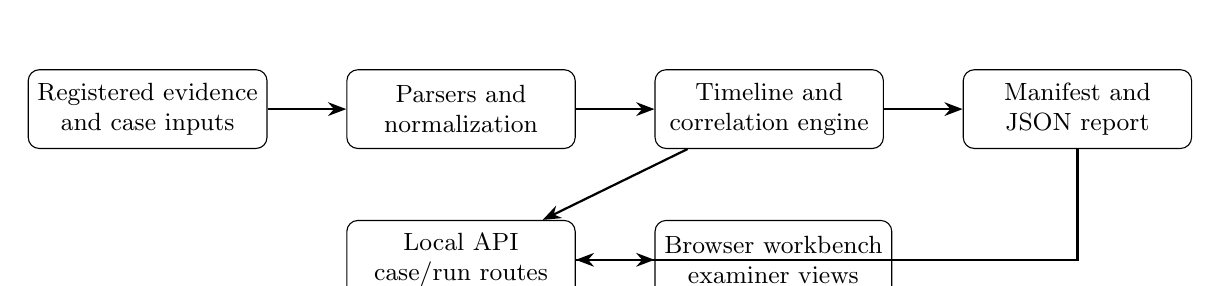
\begin{tikzpicture}[node distance=9mm and 10mm, every node/.style={font=\small}, box/.style={draw,rounded corners,align=center,minimum width=29mm,minimum height=10mm}, arrow/.style={-{Stealth},thick}]
\node[box] (files) {Registered evidence\\and case inputs};
\node[box,right=of files] (parse) {Parsers and\\normalization};
\node[box,right=of parse] (engine) {Timeline and\\correlation engine};
\node[box,right=of engine] (report) {Manifest and\\JSON report};
\node[box,below=of parse] (api) {Local API\\case/run routes};
\node[box,right=of api] (ui) {Browser workbench\\examiner views};
\draw[arrow] (files)--(parse);
\draw[arrow] (parse)--(engine);
\draw[arrow] (engine)--(report);
\draw[arrow] (engine)--(api);
\draw[arrow] (report)|-(api);
\draw[arrow] (api)--(ui);
\end{tikzpicture}
\caption{Chronicle pipeline at a functional level. Network PCAP decoding occurs in the external extractor before the structured records enter Chronicle.}
\end{figure}

\section{Network evidence provenance}
\begin{figure}[H]
\centering
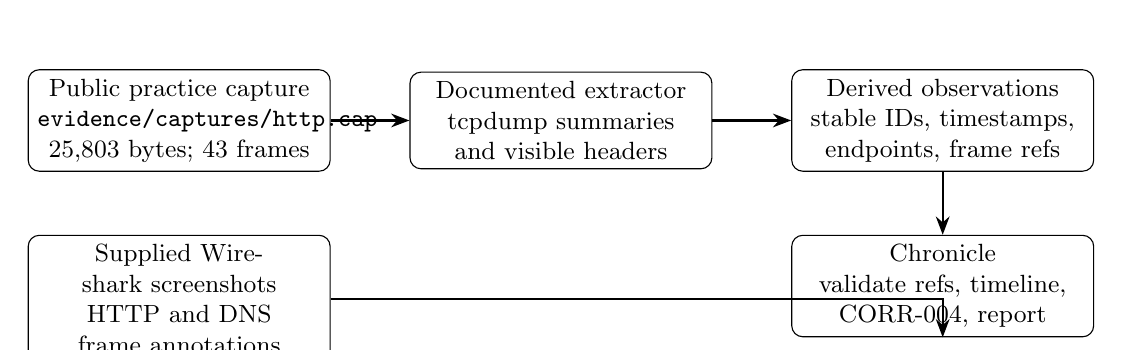
\begin{tikzpicture}[node distance=8mm and 10mm, every node/.style={font=\small}, box/.style={draw,rounded corners,align=center,text width=36mm,minimum height=11mm}, arrow/.style={-{Stealth},thick}]
\node[box] (pcap) {Public practice capture\\\texttt{evidence/captures/http.cap}\\25,803 bytes; 43 frames};
\node[box,right=of pcap] (extract) {Documented extractor\\tcpdump summaries and visible headers};
\node[box,right=of extract] (json) {Derived observations\\stable IDs, timestamps, endpoints, frame refs};
\node[box,below=of json] (chron) {Chronicle\\validate refs, timeline, CORR-004, report};
\node[box,below=of pcap] (exhibits) {Supplied Wireshark screenshots\\HTTP and DNS frame annotations};
\draw[arrow] (pcap)--(extract);
\draw[arrow] (extract)--(json);
\draw[arrow] (json)--(chron);
\draw[arrow] (exhibits)-|(chron);
\end{tikzpicture}
\caption{Network case data flow and exhibit boundary. Screenshot annotations are separate attributed exhibits; they are not decoded packet records.}
\end{figure}

\section{Examination procedure}
The reproducible flow is: (1) register the selected case and its material; (2) calculate current SHA-256 values; (3) for the network case, validate export/capture digest and frame references; (4) parse the structured records and normalize timestamps; (5) sort records into a timeline; (6) apply enabled correlation rules; (7) resolve finding references to source events; and (8) save and read back the JSON report. The extractor command and application setup are listed in Chapter 4.

\section{Integrity and time handling}
The capture SHA-256 recorded in the current report is \texttt{25a72bdf10339f2c29916920c8b9501d294923108de8f29b19aba7cc001ab60d}. Chronicle compares the current capture fingerprint with the digest embedded in the derived export. No independent trusted acquisition-time baseline was supplied. Recalculation therefore demonstrates consistency of current files, not historical authenticity or custody. Packet epoch times are rendered as UTC; the capture's original timezone context was not independently established. UTC normalization is a representation choice, not verification of the acquisition clock.

\chapter{Installation and Setup}
\section{Requirements}
The repository uses Python with dependencies listed in \texttt{requirements.txt}, Node.js/npm for the frontend, and tcpdump for regenerating the network observation export. A virtual environment and frontend dependencies must already be installed. Exact versions on the submission machine should be recorded in the final recording/setup screenshot.

\section{Run locally}
From the repository root:
\begin{verbatim}
python3 -m venv .venv
.venv/bin/pip install -r requirements.txt
.venv/bin/python data/extract_http_cap.py
.venv/bin/uvicorn src.api:app --host 127.0.0.1 --port 8000
\end{verbatim}
In a second terminal:
\begin{verbatim}
cd frontend
npm install
npm run dev -- --host 127.0.0.1
\end{verbatim}
Open \url{http://127.0.0.1:5173}. The API health route is \url{http://127.0.0.1:8000/api/health}. The packet extractor is required only when rebuilding the structured network export. Commands that install packages require network access; do not run them during the demonstration if dependencies are already present.

\section{Evaluation command}
Run \texttt{.venv/bin/python evaluation/run\_evaluation.py} from the repository root. On 21 October 2026, the current repository evaluation completed 50 tests with no failures. This is evidence of tested software behavior only, not validation of the accuracy of forensic conclusions.

\chapter{Experimentation and Results}
\section{Network practice examination}
The capture is PCAP 2.4 with Ethernet link type, 25,803 bytes, and 43 frames. The recorded current digest is shown above. The derived export contains 43 observations with unique frame references. Chronicle's generated report records successful provenance checks for capture presence, matching export digest, observation digest references, unique/in-range frame numbers, source-reference consistency, and frame count.

\begin{longtable}{p{0.10\textwidth}p{0.22\textwidth}p{0.36\textwidth}p{0.22\textwidth}}
\caption{Selected source observations from the public practice capture}\\
\toprule Frame & Timestamp (capture-relative) & Observation & Reference\\
\midrule
\endfirsthead
\toprule Frame & Timestamp (capture-relative) & Observation & Reference\\
\midrule
\endhead
4 & 0.911310 s & Client requests \texttt{/download.html}; supplied notes identify Host \texttt{www.ethereal.com}. User-Agent is client-reported text. & Capture frame 4; HTTP exhibit\\
13 & 2.553672 s & DNS A query for \texttt{pagead2.googlesyndication.com}. & Capture frame 13; DNS exhibit\\
17 & 2.914190 s & Response shares transaction ID \texttt{0x0023} and reversed endpoints; answer records are decoded in the examination notes. & Capture frame 17; DNS exhibit\\
18 & 2.984291 s & Request for \texttt{/pagead/ads}; decoded request includes the Ethereal page URL. & Capture frame 18; HTTP exhibit\\
27 & 3.955688 s & Wireshark screenshot labels this frame \texttt{HTTP/1.1 200 OK (text/html)}. & Capture frame 27; HTTP exhibit\\
38 & 4.846969 s & Wireshark screenshot labels this frame \texttt{HTTP/1.1 200 OK}. & Capture frame 38; HTTP exhibit\\
\bottomrule
\end{longtable}
The values in the timestamp column are capture-relative display times from the supplied Wireshark exhibits. Chronicle also records the packet epoch and UTC normalization. The report generated by the project gives full normalized timestamps and frame references.

\section{Finding and traceability}
The case produces one informational finding, \texttt{CORR-004}, titled “DNS query and response share a transaction.” It links event \texttt{PCAP-E0013} at \texttt{evidence/captures/http.cap\#frame=13} and \texttt{PCAP-E0017} at \texttt{evidence/captures/http.cap\#frame=17}. The records carry timestamps 2004-05-13 10:17:09.864896 UTC and 10:17:10.225414 UTC, respectively. The explanation cites matching transaction ID 35 (hexadecimal \texttt{0x0023}) and reversed endpoints. The finding's alternative explanation is ordinary DNS resolution associated with the captured webpage. The report explicitly says this does not establish malicious activity, identify a person, or prove later HTTP traffic was caused by the DNS response.

\section{Decoder reconciliation}
The supplied Wireshark HTTP filter screenshot lists frames 4, 18, 27, and 38. The local tcpdump summary heuristically labels HTTP on additional adjacent TCP segments and reports HTTP response status at frames 6, 26, and 36. The implementation preserves the distinct sources and documents this decoder/reassembly difference rather than treating them as identical output. A fresh Wireshark examination is needed if detailed stream reassembly is required.

\section{Synthetic pipeline checks}
Operation Glasshouse deterministically generates 240 event records (seed 1901). The current saved report contains 15 rule matches. The generator includes a sequence resembling repeated authentication failures, a login, file activity, archive creation, and a nearby upload observation. A scheduled service-account backup also matches the archive-to-upload rule and is a deliberate competing explanation. These synthetic patterns demonstrate rule execution and the need to evaluate alternatives; they do not provide real-world ground truth. The six-event \caseid{CHRONICLE-DEMO-001} remains a separate small regression dataset.

\section{Screenshots}
Figures below are supplied source exhibits from Shreya's workflow. The examiner must add genuine application screenshots of the running Chronicle UI and its report before final submission. The reserved capture slots are visibly marked to prevent placeholders from being represented as evidence.
\begin{figure}[H]\centering
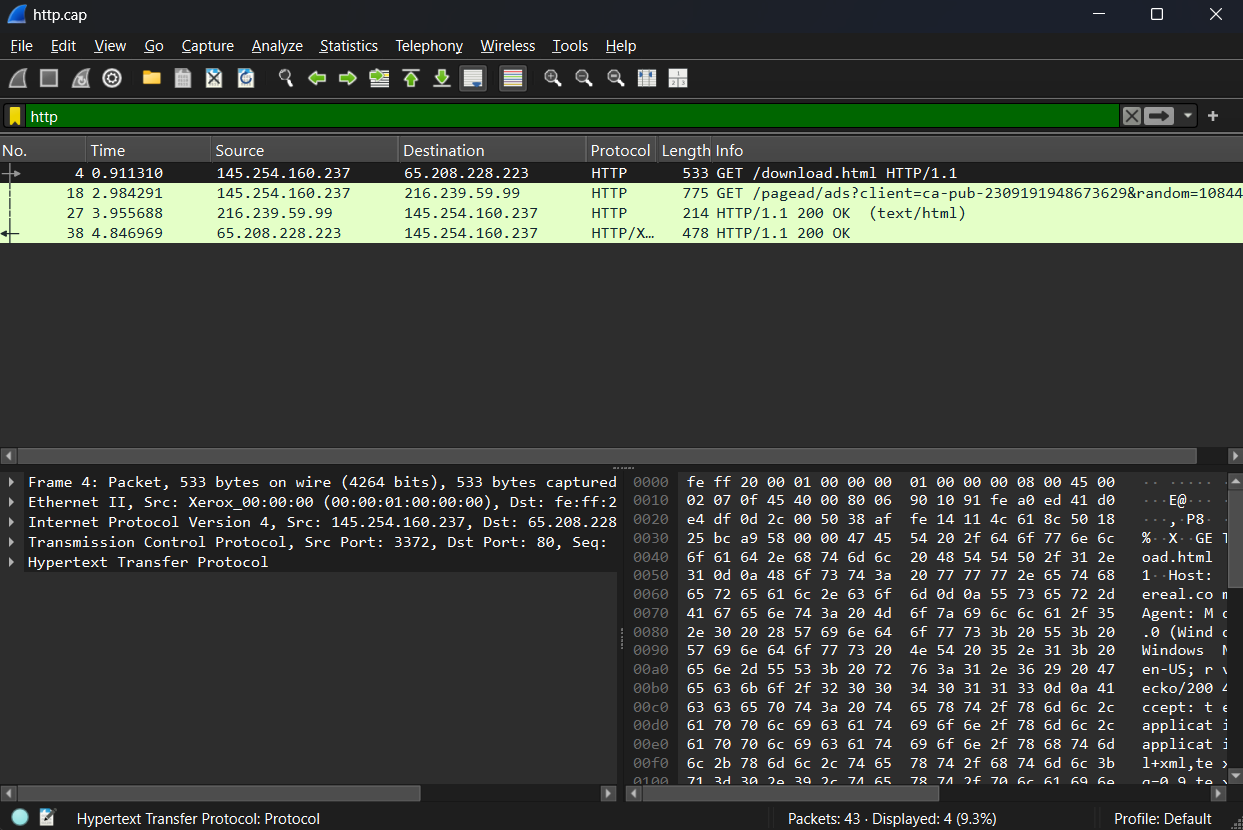
\includegraphics[width=.94\textwidth,height=.43\textheight,keepaspectratio]{images/wireshark-http.png}
\caption{Supplied Wireshark HTTP-filter screenshot. Exhibit supplied with Shreya's practice-capture materials; it documents visible filter observations, not a Chronicle screen.}\end{figure}
\begin{figure}[H]\centering
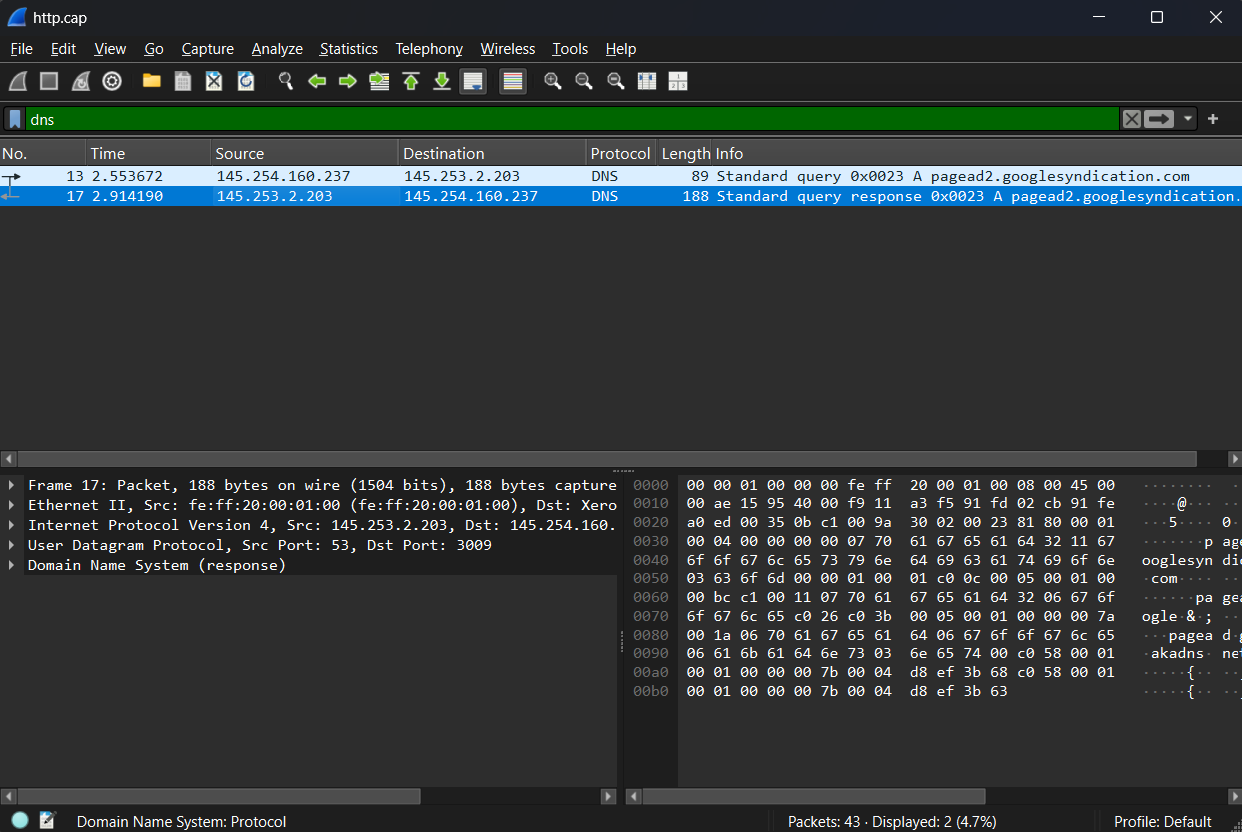
\includegraphics[width=.94\textwidth,height=.43\textheight,keepaspectratio]{images/wireshark-dns.png}
\caption{Supplied Wireshark DNS-filter screenshot. Frames 13 and 17 support the query/response observation as documented in the analysis notes.}\end{figure}
\begin{figure}[H]\centering
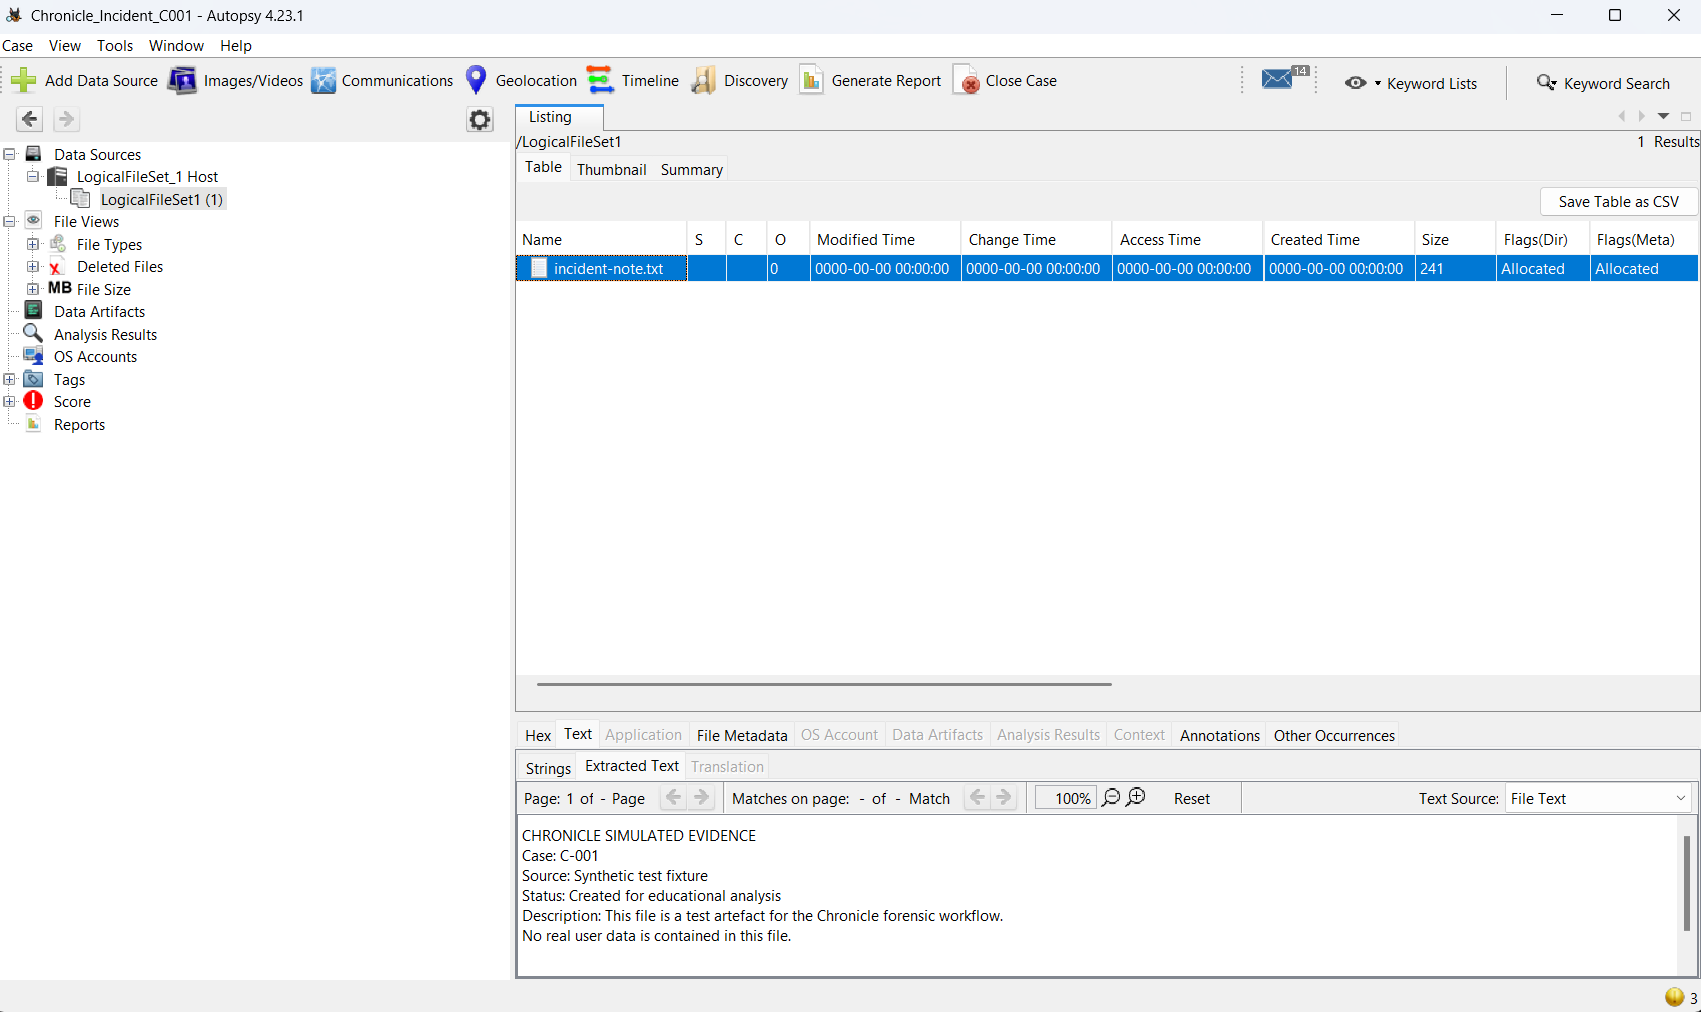
\includegraphics[width=.94\textwidth,height=.43\textheight,keepaspectratio]{images/autopsy-evidence.png}
\caption{Supplied Autopsy screenshot of a logical-file-set item and synthetic C-001 note. This is an exhibit only; Chronicle did not examine a disk image.}\end{figure}
\begin{figure}[H]\centering
\fbox{\parbox[c][45mm][c]{.88\textwidth}{\centering \textbf{Replace before submission}\\Capture the running Chronicle Network Examination page with the 43 observations and source references visible.\\Use an unedited screenshot from the actual application.}}
\caption{Reserved Chronicle application screenshot slot; not evidence until replaced with a real capture.}\end{figure}
\begin{figure}[H]\centering
\fbox{\parbox[c][45mm][c]{.88\textwidth}{\centering \textbf{Replace before submission}\\Capture the generated CORR-004 finding and its two source-record/frame references in Chronicle.}}
\caption{Reserved traceability screenshot slot; not evidence until replaced with a real capture.}\end{figure}
\begin{figure}[H]\centering
\fbox{\parbox[c][45mm][c]{.88\textwidth}{\centering \textbf{Replace before submission}\\Capture the generated investigation report or report export in Chronicle.}}
\caption{Reserved report screenshot slot; not evidence until replaced with a real capture.}\end{figure}

\chapter{Analysis of Outcome}
\section{What an examiner can do}
Within the registered local cases, an examiner can select a case, run the pipeline, review the evidence inventory and file hashes, inspect parsed records and timeline entries, inspect rule matches and supporting records, and obtain a generated JSON report. In the network case, that workflow is useful because a single lead can be followed to two frame-level source references and their timestamps. Repeatability is supported by stable export event IDs and documented extraction steps.

\section{Traceability assessment}
For generated findings, the current report contains supporting event IDs, source IDs, timestamps, and source references. The network lead resolves to frames 13 and 17. The pipeline validation also checks that report references resolve. This is meaningful record-level traceability for the supplied structured input. It is not equivalent to independent reproduction of every protocol decode: the source export is externally generated, Wireshark screenshot annotations are visual exhibits, and decoder behavior differs on some frames. A report reader should consult the capture and exhibit for the underlying packet-level detail.

\section{Integrity and attribution}
SHA-256 supports comparison of current bytes against a known digest. Because the project lacks an independently acquired trusted baseline and a complete chain-of-custody record, the displayed fingerprint does not establish where or when the file was acquired or whether it was altered before the baseline. Network endpoints and a client-reported User-Agent are not proof of a human user. No attribution conclusion is supported by this practice capture.

\section{Three main functional weaknesses}
\begin{enumerate}
\item \textbf{Network parsing depends on a derived export.} Chronicle does not ingest and decode PCAP natively. Reproduction and deeper protocol/stream analysis require external tooling and careful preservation of the export-to-capture relationship.
\item \textbf{Evidence intake and case management are fixed.} There is no general case-creation/upload workflow, partial-record quarantine, or complete acquisition and custody ledger. The current demonstration works on repository-registered cases.
\item \textbf{Finding review is rule-led and bounded.} Rules surface associations but cannot establish authorization, identity, causation, or intent. The UI and JSON report provide traceability for current records, but richer examiner notes, source-level validation, uncertainty management, and broader artifact adapters remain future work.
\end{enumerate}

\chapter{Conclusion and Future Work}
Chronicle currently provides a defensible, executable academic demonstration when its scope is stated accurately. Its strongest story follows Shreya's public network practice material into a structured, source-linked Chronicle examination, then uses the independent Glasshouse synthetic case to demonstrate event correlation and competing explanations. The network output is one ordinary DNS query/response informational lead; the available material supports no claim of attack or user attribution. C-001 and the Autopsy screenshot remain separate, and no disk-image analysis is claimed.

The smallest high-value next implementation is to improve source-to-finding examination in the network case: keep each observation's packet frame, exact timestamp, endpoints, decoded fields, exhibit provenance, and interpretation together in an examiner view and export. The current build has much of this data, so the remaining work should focus on making the path from finding to record to source unmistakable, capturing genuine app screenshots, and ensuring the report is reproducible. Longer-term work includes native PCAP ingestion or a validated adapter contract, acquisition metadata and custody events, user-created cases, partial parse-error handling, structured Autopsy exports, and richer rule evaluation. Those extensions should be pursued only with test evidence and suitable source material.

\chapter{Team Participation}
The project team comprises Neil, Shreya, and Aarohi. The presentation gives each person a speaking segment to satisfy the assignment's participation requirement. The speaking allocation is not an attribution of implementation work.
\begin{itemize}
\item \textbf{Shreya:} Confirmed contribution of the public Wireshark practice capture, HTTP/DNS analysis notes and screenshots, Autopsy screenshot, and incident/evidence-integrity materials.
\item \textbf{Aarohi:} Team member and presentation participant. The available project context does not establish a specific component contribution; no specific implementation responsibility is asserted.
\item \textbf{Neil:} Team member and presentation participant. The available project context does not establish a specific component contribution; no specific implementation responsibility is asserted.
\end{itemize}
Each member should review and personalize their narration to reflect what they actually did. Do not retain a speaking allocation as a claim of authorship.

\chapter{References}
\begin{enumerate}[label={[}\arabic*{]}]
\item National Institute of Standards and Technology, \emph{Guide to Integrating Forensic Techniques into Incident Response}, NIST SP 800-86, 2006. \url{https://csrc.nist.gov/pubs/sp/800/86/final}
\item National Institute of Standards and Technology, \emph{Secure Hash Standard (SHS)}, FIPS PUB 180-4, 2015. \url{https://csrc.nist.gov/pubs/fips/180-4/upd1/final}
\item P. Mockapetris, \emph{Domain Names -- Implementation and Specification}, RFC 1035, IETF, 1987. \url{https://www.rfc-editor.org/rfc/rfc1035}
\item tcpdump project, \emph{tcpdump manual page}. \url{https://www.tcpdump.org/manpages/tcpdump.1.html}
\item Chronicle project repository, source code and supporting documents: \texttt{src/}, \texttt{data/}, \texttt{docs/}, \texttt{tests/}, and generated case reports. Local project artifact, accessed 21 October 2026.
\item Supplied public Wireshark practice capture and analysis materials: \texttt{evidence/captures/http.cap}, \texttt{docs/investigation/wireshark-analysis.md}, and \texttt{evidence/screenshots/}. Contribution and provenance recorded in \texttt{docs/evidence-provenance.md}.
\item Course assignment sheet, \emph{CFL (H) IA Sem-V 2026--27}, Cyber Forensics \& Laws, course 216H02C501, July--November 2026; and IA\#2 rubric screenshot supplied by the team.
\end{enumerate}

\appendix
\chapter{Reproducible Demonstration Checklist}
The accompanying video script in \texttt{docs/demo-script.md} assigns one continuous speaking block to each presenter in this order: Neil, Shreya, then Aarohi. The total target duration is 7 minutes 30 seconds, within the required 7--8 minute window.
\begin{enumerate}
\item Start the API and frontend using Chapter 4 commands.
\item Select \caseid{WIRESHARK-PRACTICE-001} and run the investigation.
\item Show the capture fingerprint and its no-independent-baseline caveat.
\item Inspect frames 13 and 17 in the network observation view.
\item Open \texttt{CORR-004} and follow both source records back to frame references.
\item Open the generated report and explain the alternative interpretation and limitations.
\item Show the Autopsy screenshot only as a synthetic C-001 exhibit.
\item Switch to \caseid{OPERATION-GLASSHOUSE} and explain that its 240 records are generated and separate.
\item Record all three members within a total duration of 7--8 minutes.
\end{enumerate}

\chapter{Final Submission Completion Checks}
\begin{itemize}
\item Fill the three roll numbers and verify official institution, department, course code, instructor spelling, and dates.
\item Replace all three Chronicle screenshot placeholders with genuine, unedited captures from the running application.
\item Verify all figures remain legible in the final PDF and retain the source capture provenance.
\item Ensure the final recording is between 7 and 8 minutes and includes Neil, Shreya, and Aarohi.
\item Submit the report, recording, and GitHub Classroom repository using the course's specified submission channels.
\end{itemize}
\end{document}
